\chapter{Building productivity mobile application}

\begin{wrapfigure}[16]{r}[0pt]{0.3\linewidth}
   \centering
	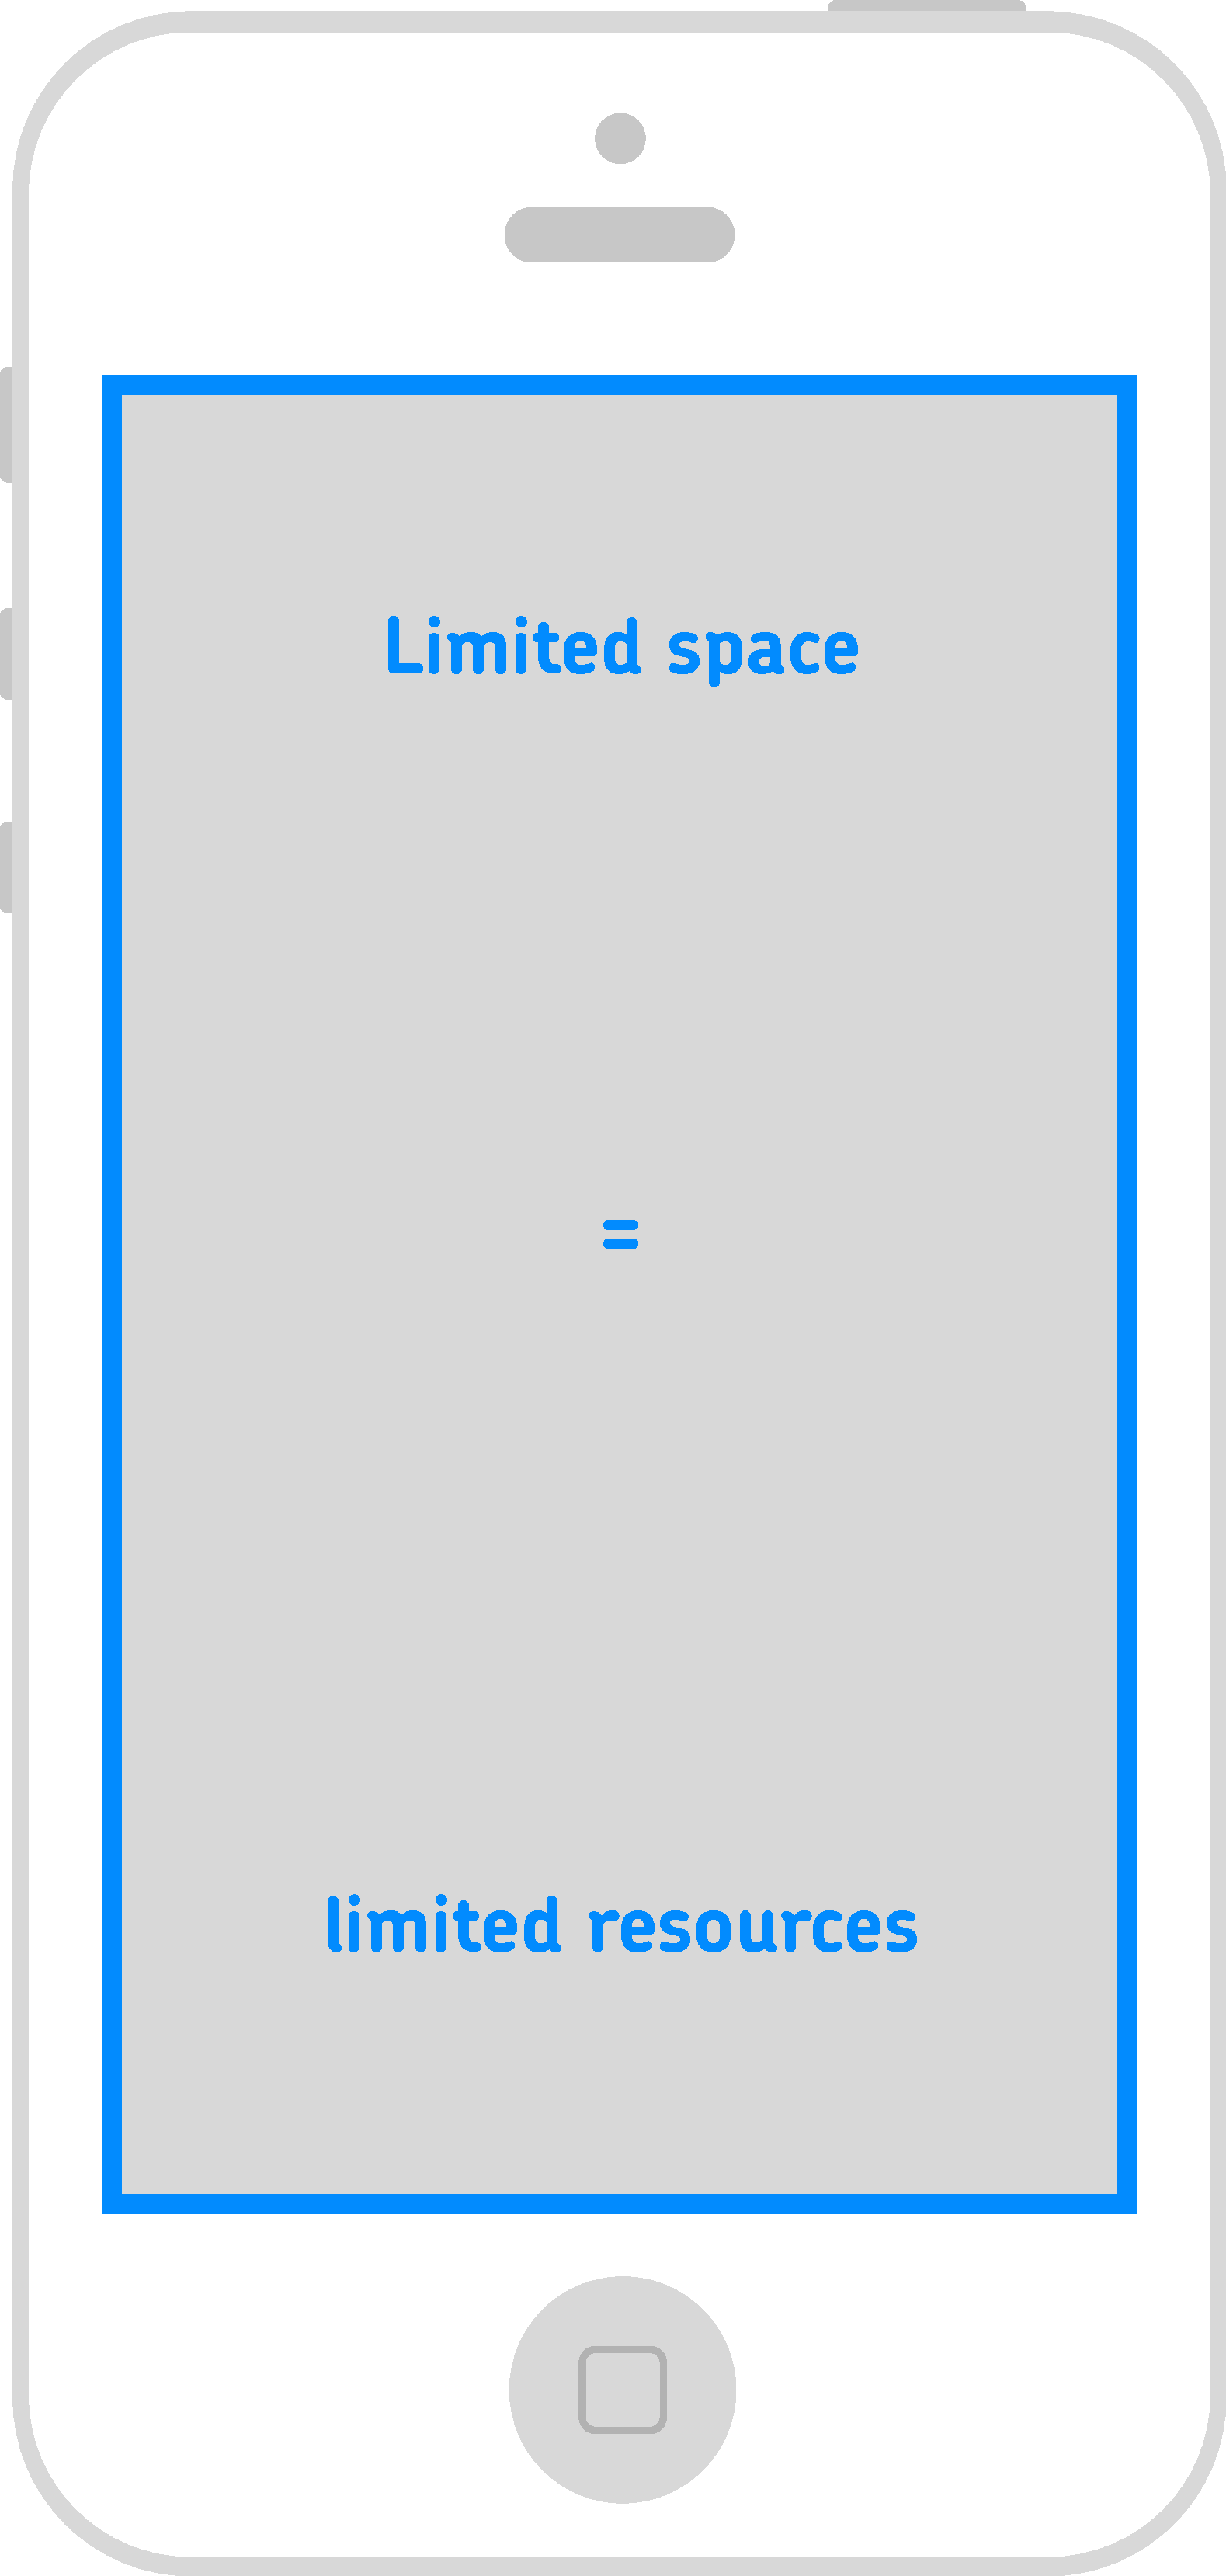
\includegraphics[width=1\linewidth]{resources/limited-resources.pdf}
	\caption[Happy Perform, limited space and resources]{Happy Perform, limited space and resources}
\end{wrapfigure}

In this chapter the prototype of personal performance mobile application will be considered. Let's call it ``Happy Perform'' (\url{happy-perform.com})

\section{Abstractions and games}
There is an important notion of feedback within the concept of ``Flow'' and appearing in all of the method of project management.

The only application from considered ones in chapter \ref{chap:apps} did try to use a concept of feedback: ``Carrot''. It used a game mechanic called ``Negative reinforcement'' in order to state a bad system condition: there is a lot of tasks, that require attention.

\begin{figure}
   \centering
	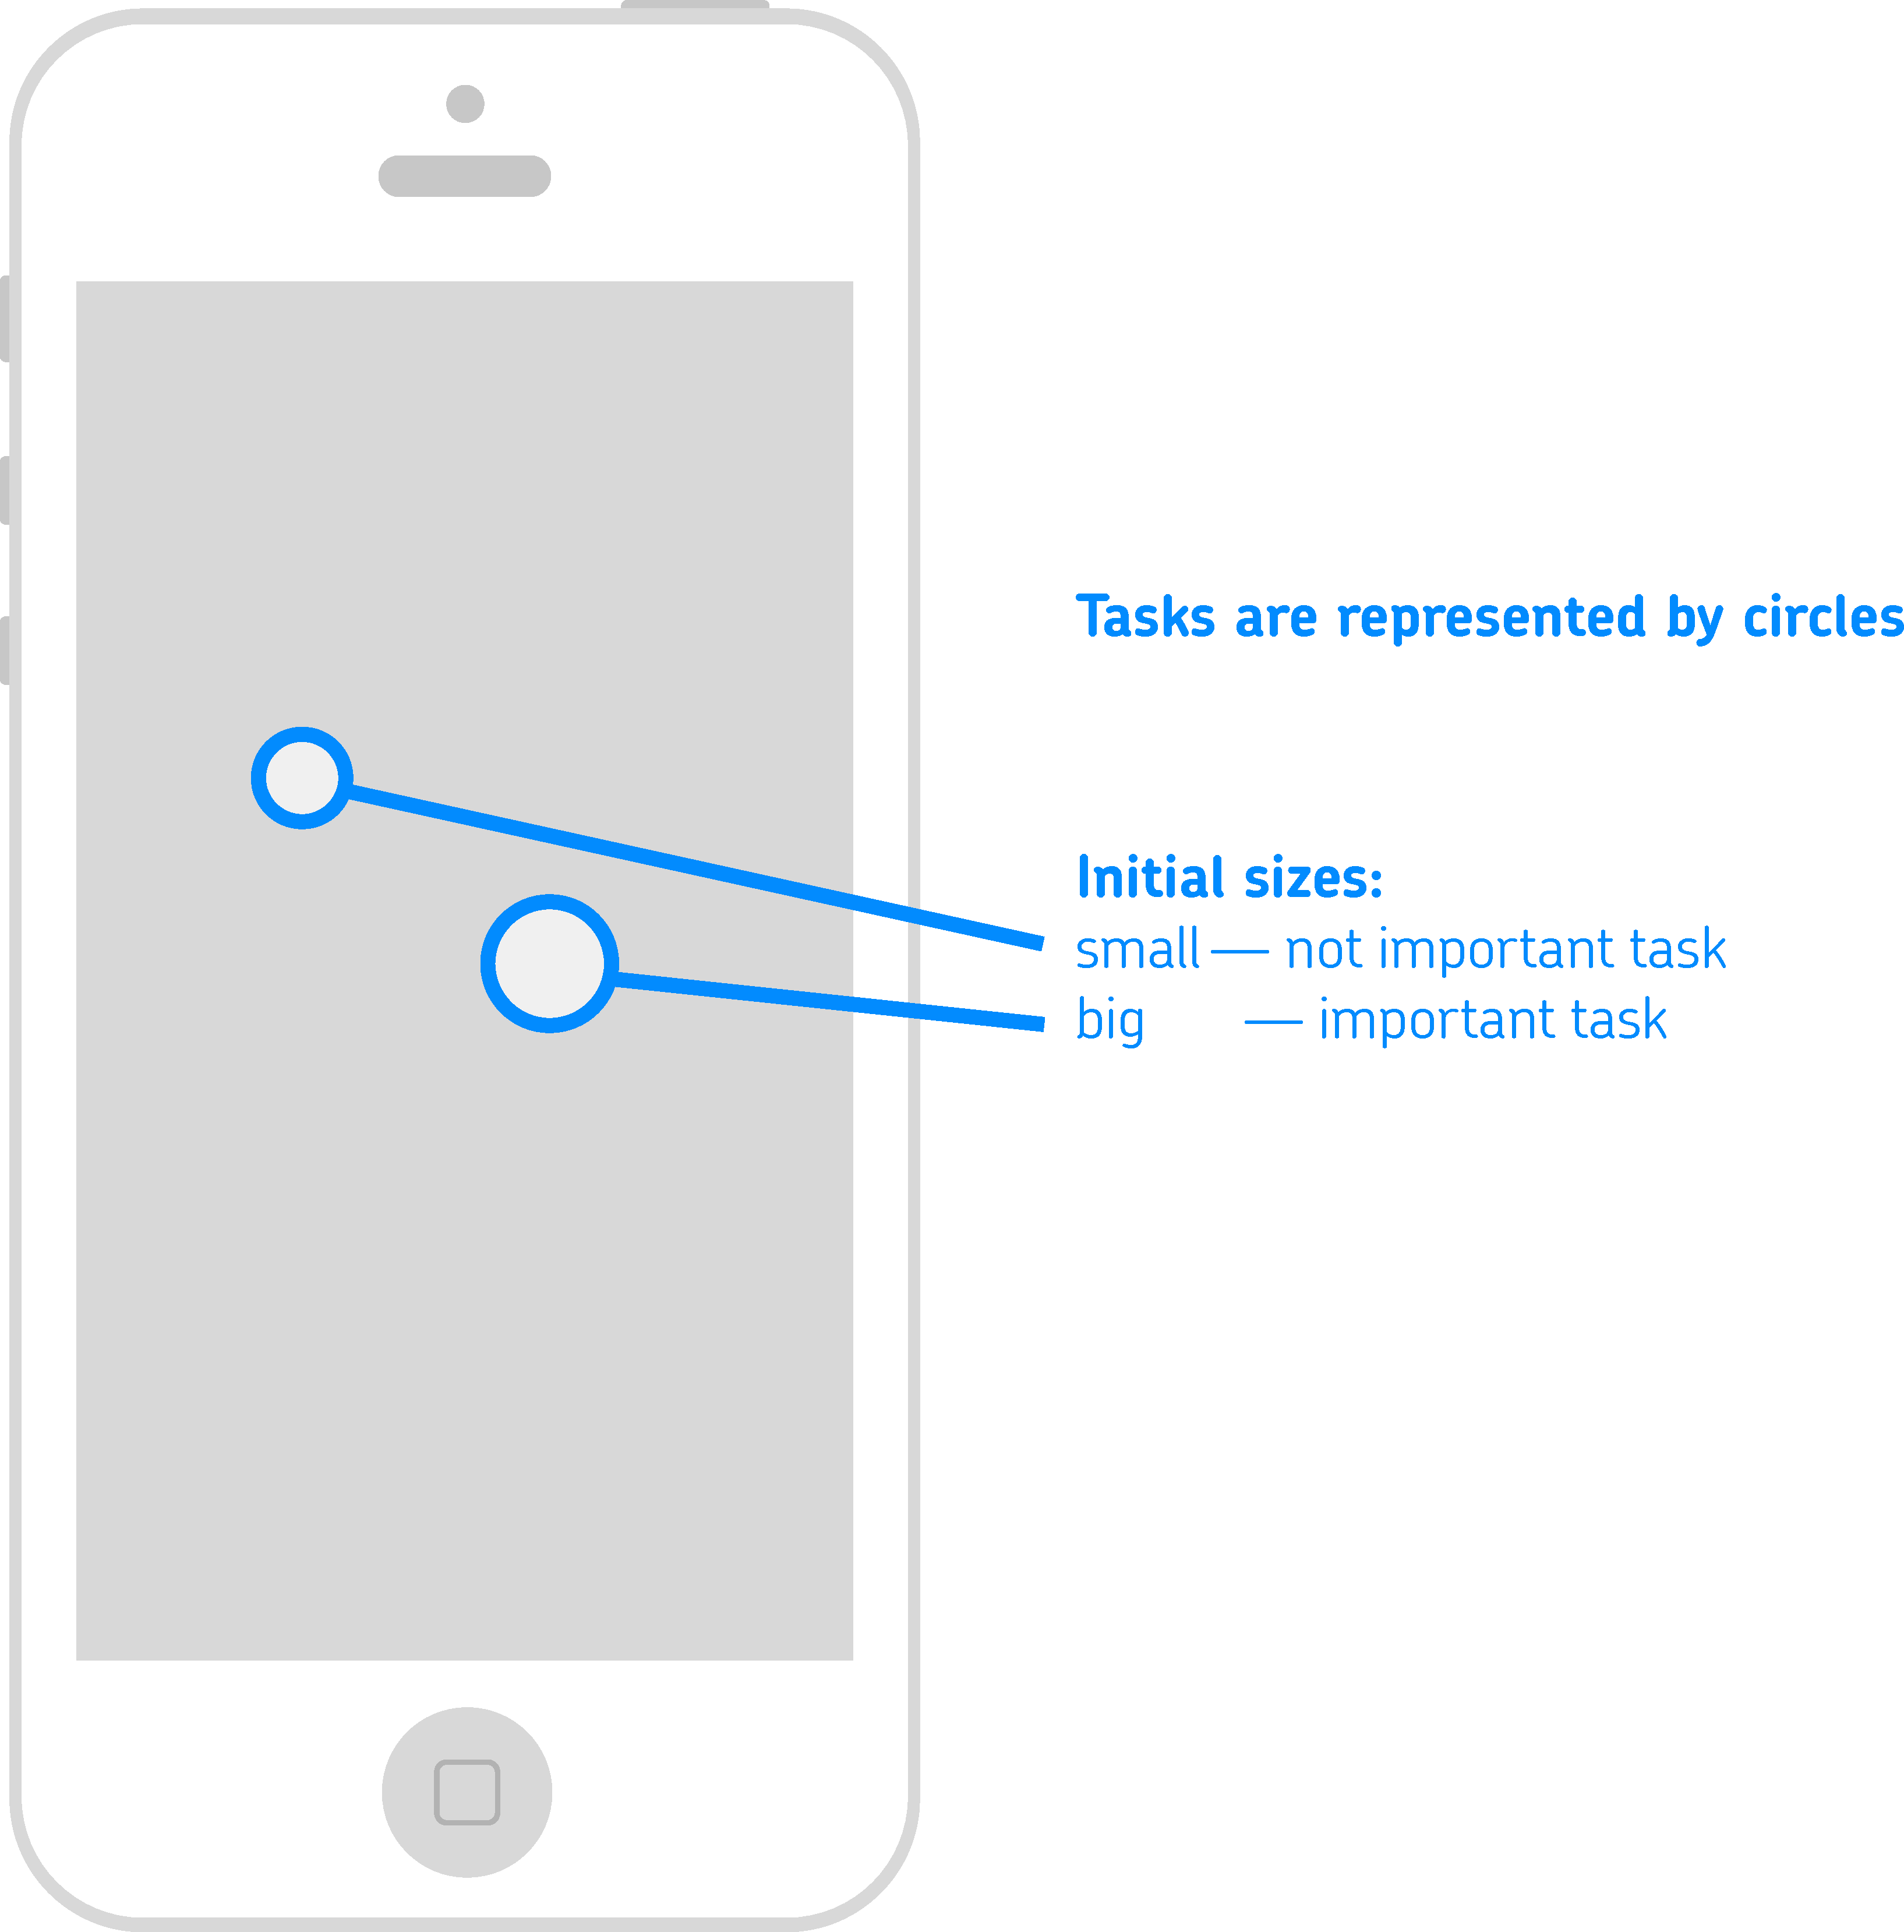
\includegraphics[width=0.8\linewidth]{resources/tasks.pdf}
	\caption[Happy Perform, tasks representation]{In Happy Perform tasks are represented by circles}
\end{figure}

\subsection{Concept of time limitation}

Each task (that has a deadline) can be represented as a system with dynamic complexity. As focus is a limited resource, as a time, tasks that don't get enough attention can lead to a bad state of a system very fast. Thus causing lack of time and lack of focus, which recursively make situation even worse.

Listed application didn't use the concept of limited resource. One of the ways to illustrate the limited resource was introduced by popular games: bubbles and tetris.

Using a mobile screen as limitation to available tasks, it is possible to construct the following abstraction:

\begin{compactitem}
\item The vertical axis represents time available till deadline
\item The space represents required focus and illustrates which tasks require immediate action
\item Each can be represented as a circle, initial (normal) size of the circle is determined by its importance (important or not)
\item Space can also group related tasks
\end{compactitem}

\section{Game mechanics in use}

In the case of application there are two main dynamics used:

\begin{compactenum}
\item Appointment Dynamic, which requires to return at a predefined time to mark a task as ``in progress'' or ``complete''.\item Using disincentives to illustrate limited space: if there is not enough space, it is impossible to add new task
\end{compactenum}

\begin{figure}
   \centering
	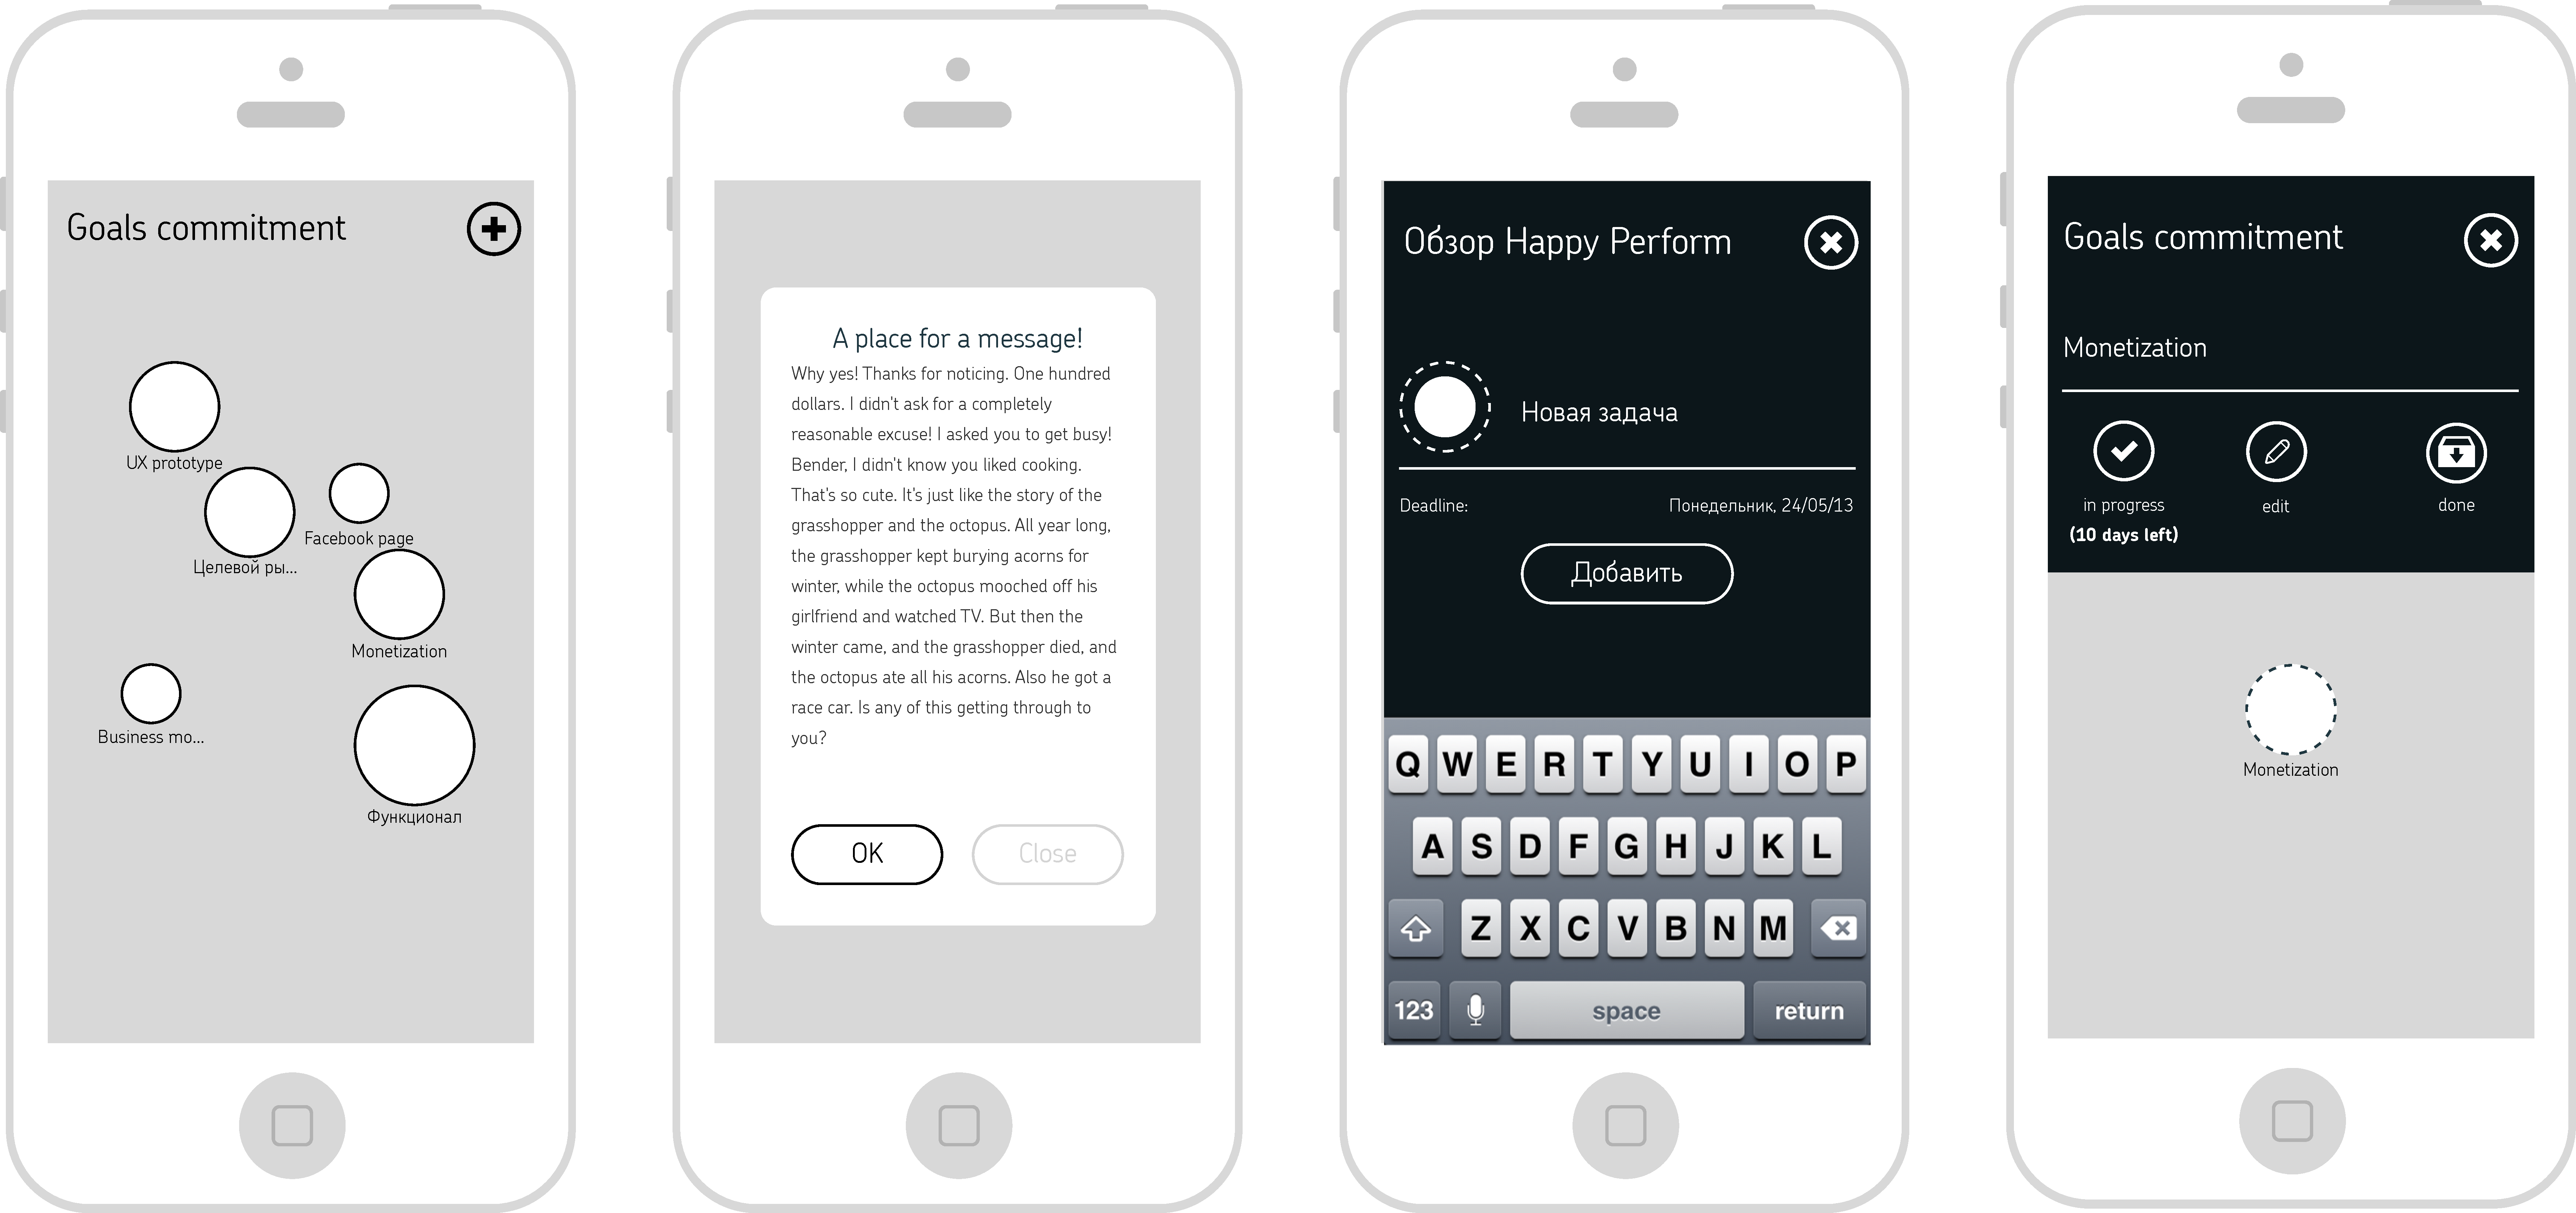
\includegraphics[width=1\linewidth]{resources/other-screens.pdf}
	\caption[Happy Perform, other screens]{Happy Perform: tasks list, message bubble, adding a task, task options}
\end{figure}

\section{Application workflow}

Let's assume a person have a number of tasks. It is possible to classify them in a following way: 
\begin{compactenum}
\item recurring tasks
\item tasks with deadlines set too far (e.g.: buy a flat)
\item tasks with deadlines not yet defined
\item tasks with defined start date (e.g.:tuesday, movie)
\item \em ``frogs'', or tasks that are worst or most important (they can be recurring, or anything else)
\end{compactenum}

Those can be grouped into two categories: continuous and instant. Continuous tasks require recurring ``in progress'' mark. Instant tasks don't have deadlines.

Let's fill in those tasks into ``Happy Perform'' application. ``Frogs'' will get an `important' status and a bigger circle size.

Deadlines are very important. Also setting a KPI (key performance indicator) to a task is effective: it gives a required feedback. The universal KPI in the case of ``Happy Perform'' is the size of the circle and position on the screen: tasks start from the top with a certain speed (that is defined with the number of days till deadline) and move towards bottom of the screen, at the day of deadline they will reach the bottom.

Instant tasks (that should be done `today') appear at the bottom of the screen initially.

Each day a person should mark tasks he did as ``in progress'' or they will start to grow exponentially. An oversized task start to shrink to initial size if marked as ``in progress''. Tasks on the bottom will grow even if mark as ``in progress'', but slower.

There is no mechanism to manage recurring tasks and defined start date tasks in the first version of application.

This concept will be produced and tested as a part of a complex productivity solution.


